\documentclass[12pt,oneside,a4paper,english]{article}
\usepackage[T1]{fontenc}
\usepackage[margin=2.25cm,headheight=26pt,includeheadfoot]{geometry}
\usepackage{listings}
\usepackage{color}
\usepackage{titlesec}
\usepackage{titling}
\usepackage[framed, numbered]{matlab-prettifier}
\usepackage{changepage}
\usepackage{amsmath}
\usepackage{hyperref}
\usepackage{enumitem}
\usepackage{graphicx}
\usepackage{fancyhdr}
\usepackage{lastpage}
\usepackage{caption}
\usepackage{tocloft}
\usepackage{setspace}
\usepackage{multirow}
\usepackage{titling}
\usepackage{float}
\usepackage{comment}
\usepackage{booktabs}
\usepackage{indentfirst}
\usepackage{lscape}
\usepackage{booktabs,caption}
\usepackage[flushleft]{threeparttable}
\usepackage[english]{nomencl}
\usepackage{xcolor}
\usepackage{lipsum}
\usepackage[utf8]{inputenc}
\usepackage[english, danish]{babel}
\usepackage{longtable}
\usepackage{csquotes}
\usepackage[toc,page]{appendix}

\usepackage[style=authoryear,sorting=nty]{biblatex}
\addbibresource{references.bib}


% --- set footer and header ---
\pagestyle{fancy}
\fancyhf{}

\setlength{\parindent}{0em}
\title{CDIO del 3} % to reference as \title, dont use \maketitle
\makeatletter\let\Title\@title\makeatother



\lstset{language=Matlab,
style=Matlab-editor,
basicstyle=\normalsize\mlttfamily,
numbers=left,
numberstyle={\scriptsize\color{black}},			% size of the numbers
numbersep=0.5cm											
}

\newlist{steps}{enumerate}{1}
\setlist[steps, 1]{leftmargin=1.5cm,label = Step \arabic*:}
\renewcommand{\headrulewidth}{1pt}
\renewcommand{\footrulewidth}{1pt}

%\lhead{\Title}
\rhead{\nouppercase{\rightmark}}
\lhead{\Title}
\rfoot{
\includegraphics[height=1.25cm]{root/logo.pdf}} % right header logo
\setlength\headheight{16pt}
\setlength{\footskip}{50pt}
\lhead{\Title} %rightH title
\cfoot{\thepage}

% --- End of page settings ---



\begin{document}
\pagenumbering{roman} 

\begin{titlepage}
\begin{center}
%\textsc{ Danmarks Tekniske Universitet}\\[1.5cm]

\includegraphics[width=0.4\textwidth]{root/dtu.png}
\vspace{1cm}

02312

INDLEDENDE PROGRAMMERING

\vspace{.5cm}

% Title
\hrule
\vspace{.5cm}
{ \huge \bfseries CDIO Final} % title of the report
\vspace{.3cm}\linebreak
\url{https://github.com/Oliver-Olsen/matador3ugers}
\vspace{.3cm}
\hrule
\vspace{.5cm}

\textsc{\textbf{Authors}}\\
\vspace{.5cm}


\begin{tabular}[!c]{cccc}
  Krzysztof Kisiel s192884 & 
\includegraphics[width=2.75cm]{root/krzysztof.png} &   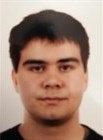
\includegraphics[width=2.75cm]{root/oliver.png} & Oliver Olsen s205443  \\

 Johannes Jensen
s205413 & 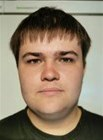
\includegraphics[width=2.75cm]{root/johannes.png} &   
\includegraphics[width=2.75cm]{root/gustav.PNG} & Gustav Fauser s205446 \\

Jonathan Hansen	
s205415 &
 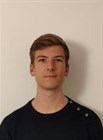
\includegraphics[width=2.75cm]{root/jonathan.png} &   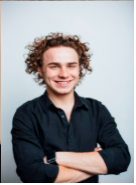
\includegraphics[width=2.75cm]{root/alaa.PNG} & Alaa Hadood 
s205477 \\

\end{tabular}

\vspace{.5cm}
\centering \today % Dags dato
\end{center}
\end{titlepage}


\newpage
\pagenumbering{arabic} 
%\fancyhead[C]{Side \thepage\ af \pageref{LastPage}}

\fancyfoot[C]{Side \thepage\ af \pageref{endOfDoc}}

\rhead{Timeplan \& Summary}
\section{Timeplan} \label{ch1}
\begin{table}[H]
\begin{tabular}{lccccc}
\hline
\multicolumn{1}{|l|}{Tid i timer} & Krav og analyse & \multicolumn{1}{l}{Design} & Implementering & Test & Programmering \\ \cline{2-6} 
\multicolumn{1}{|l|}{Navn} &  & \multicolumn{1}{l}{} &  &  &  \\ \cline{1-1}
Gustav Fauser &0&0& 0 &0 &  0  \\
Oliver Olsen & 0& 0 &0 & 0 & 0 \\
Krzysztof Kisiel & 0 & 0 & 0 & 0 & 0  \\
Johannes Jensen & 0 & 0 & 0 & 0 & 0 \\
Jonathan H\o j & 0 & 0 & 0 & 0 & 0 \\
Alaa Hadood & 0 & 0 & 0 & 0 & 0 \\ \hline
\end{tabular}
\caption{Tabel over antal timer brugt p\aa \space hver del af projektet, for hvert enkelt medlem}
\label{table:timeplan}
\end{table}

 

\section{Summary} \label{ch2}
In this project we have created a digital version of the game "Matador". The game is implementede in Java. From the customer's vision, a list of requirements and use cases has been prepared, and used to create the program. The game has been tested in accordance to the requirements, to document that the program is meeting the requirements. 


%------------------Indholdsfortegnelse start------------------

\newpage
\rhead{Indhold}
\doublespacing
%\addcontentsline{toc}{section}{Table of Contents}
\renewcommand{\baselinestretch}{1}\normalsize
\tableofcontents
\renewcommand{\baselinestretch}{1}\normalsize
%\singlespacing
\thispagestyle{fancy} % force page style

%------------------Indholdsfortegnelse slut------------------


\newpage
\rhead{Introduktion}
\section{Introduktion} \label{ch3}
IOOuterActive (os) har fået til at opgave at designe og implementere et Monopoly  spil. Der skal implementeres de væsentligste elementer fra brætspillet, for at spillet kan spilles. Spillet skal kunne spilles mellem 2-4 spillere.
 


\rhead{Krav}
\section{Krav} \label{ch4}
For at kunne imødekomme kundens vision, er der blevet opstillet en række krav, der tilsammen skal udgøre det samlede spil. Kravene er blevet prioriteret i høj, mellem og lav. Dernæst er kravene internt i kategorierne blevet prioriteret fra højest til lavest. 


\subsection{Høj prioritet}

\begin{itemize}
    \item Spillerne skal kunne kaste med 2 terninger og flytte det viste antal felter, på brættet.
    \item En spiller vinder spillet, når alle andre spillere er udgået.
    \item En spiller udgår af spillet, hvis vedkommende skylder mere, end de ejer.
    \item Der skal være en spilleplade tilsvarende til den set på bilag 1 (billede af spillepladen).
    \item Spilleren skal kunne købe den grund, spilleren lander på, hvis den ikke ejes af en anden spiller.
    \item Spillerne skal modtage husleje, når en anden spiller lander på deres grund.
    \item Der skal kunne være mellem 2 og 6 spillere.
    \item Spillernes brikker skal fra spillets start være placeret på startfeltet.
    \item Når en spiller passerer START-feltet, modtager spilleren som udgangspunkt 4.000 kr.
\end{itemize}

\subsection{Mellem prioritet}

\begin{itemize}
    \item Der skal være et felt ved navn “Prøv lykken” hvor spilleren har mulighed for at tage et chancekort
    \item Hvis en spiller lander på “I fængsel” feltet skal de være på besøg, og ikke straffes.
    \item Hvis spilleren lander på “De Fængsles” feltet, kommer spilleren i fængsel. Ved passering af START-feltet modtager spilleren da ikke de 4.000 kr.
    \item Hvis en spiller slår to ens, får de en ekstra tur. Slår spilleren igen to ens, ryger de direkte i fængsel.
       -Hvis en spiller slår to ens, skal spilleren udføre handlingerne på begge felter.
    \item Spilleren løslades fra fængslet ved at betale en bøde på 1.000 kr.
    \item Spilleren kan løslades fra fængslet ved at slå to ens, hvilket resulterer i, at spilleren rykker det antal felter frem, som øjnene viser, og har stadig ekstra kast.
    \item Spilleren kan bruge løsladelseskortene  til at komme ud af fængslet
    \item Hvis en spiller ejer alle grunde i en farve, fordobles lejen.
    \item Spilleren skal kunne bygge huse på sine grund, hvis de ejer alle grunde i serien.
    \item Spilleren skal bygge jævnt på grunde med samme farve.
\end{itemize}

\subsection{Lav prioritet}

\begin{itemize}
    \item Spilleren skal kunne bygge et Hotel hvis de har 4 huse på hver af grundene i serien og tilstrækkeligt penge.
    \item En spiller skal kunne pantsætte en grund, hvis de ikke har tilstrækkeligt nok penge til at betale husleje.
    \item Spillere skal kunne sælge ubebyggede grund til hinanden for en accepteret pris.
\end{itemize}
 

\newpage
\rhead{Analyse}
\section{Analyse} \label{ch5}
For at kunne designe og implementere spillet, er det nødvendigt at analysere hvad og hvordan spillet skal bruges af kunden/slutbrugerne.
\subsection{Use cases}
Use cases beskriver hvordan en eventuel spiller interagere med spillet. 
\begin{figure}[h]
    \centering
    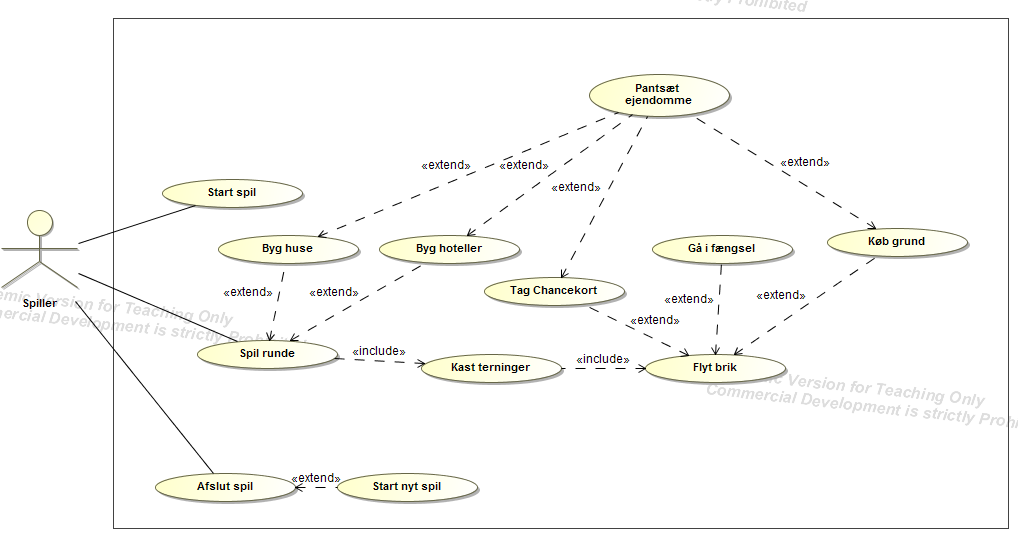
\includegraphics[width=\textwidth]{sources/5_analyse/UseCaseDiagram.PNG}
    \caption{Use case diagram}
    \label{fig:UC1}
\end{figure}

Ud fra diagrammet er der blevet udvalgt nogle kritiske use cases, som er afgørende i forhold til hvordan spillet spilles. 

\begin{itemize}
    \item Start spil
    \item Flyt brik
    \item Køb grund
    \item Gå i fængsel
    \item Tag chancekort
    \item Afslut spil
\end{itemize}

\newpage
\subsection{Use case beskrivelser}

\begin{center}
\begin{longtable}{|l|p{11cm}|}
\hline
Navn &  UC1 - Start spil\\
\hline
Short description & Spillerne starter spillet på computeren \\
\hline
Precondition & Programmet er installeret på computeren \\
\hline
Postcondition & Spillet er startet med de valgte antal spillere \\
\hline
Fejlsituationer & Ugyldigt antal spillere \\
\hline
Status i tilfælde af fejl & Spillet starter ikke \\
\hline
Aktører & Spiller \\
\hline
Udløser & Spillerne vil gerne spille spillet \\
\hline
Standard process &  
\begin{minipage}[t]{1\textwidth}
  \begin{enumerate}
      \item Spillet startes op på computeren
      \item Der vælges et antal spillere fra 2-6
      \item Der vælges navn for spillerne
      \begin{itemize}
          \item Spiller 2-6 vælger navn 
          \newline
          \emph{gentag indtil alle spiller har valgt navn}.
      \end{itemize}
      \item Der vælges farve for spillerne
      \begin{itemize}
          \item Spiller 2-6 vælger farve 
          \newline
          \emph{gentag indtil alle spiller har valgt en farve}.
      \end{itemize}
      \item Der vælges en brik til alle spillerne
      \begin{itemize}
          \item Spiller 2-6 vælger brik 
          \newline
          \emph{gentag indtil alle spiller har valgt en brik}.
      \end{itemize}
      \item Spillet starter med de valgte navne, farver og brikker.\vspace{0.5cm}
  \end{enumerate} 
  \end{minipage}
\\
\hline
Alternativ process & 
\begin{minipage}[t]{1\textwidth}
 \begin{itemize}
 \vspace{0.5cm}
     \item Der indtaster mindre eller flere spillere end 2-6
        \begin{enumerate}
            \item Spillet giver en fejlbesked
            \item Spilleren ændrer antal spillere
            \item forsætter fra 2. i hoveddelen
        \end{enumerate}
    \item Der vælges en forkert brik, eller en brik der er optaget
    \begin{enumerate}
        \item Spillet giver en fejlbesked
        \item Spilleren vælger en anden brik
        \item fortsætter fra 7. i hoveddelen
    \end{enumerate}
 \end{itemize}
\end{minipage}

\\
\hline
\end{longtable}
\end{center}



\begin{center}
\begin{longtable}{|l|p{11cm}|}
\hline
Navn &  UC2 - Flyt brik\\
\hline
Short description & Den nuværende spiller kaster terningerne og flytter sin brik \\
\hline
Precondition & Det er spillerens tur \\
\hline
Postcondition & Spilleren har taget sin tur, og turen er gået videre til den næste spiller \\
\hline
Fejlsituationer & Ingen \\
\hline
Status i tilfælde af fejl & Spilleren tager ikke sin tur \\
\hline
Aktører & Spiller \\
\hline
Udløser & Det er spillerens tur \\
\hline
Standard process &  
\begin{minipage}[t]{1\textwidth}
  \begin{enumerate}
      \item Spilleren kaster terningerne.
      \item Spilleren flytter sin brik fra det nuværende felt \newline til det næste felt.
      \begin{itemize}
          \item Spilleren lander på en grund.\newline
          \emph{Se alternativ process.} 
          \item Spilleren lander på besøg i fængsel.\newline
          \emph{Se alternativ process.}
          \item Spilleren lander på gå i fængsel.\newline
          \emph{Se alternativ process.}
          \item Spilleren lander på Prøv lykken.\newline
          \emph{Se alternativ process.}
          \item Spilleren lander på Parkering.\newline
          \emph{Se alternativ process.}
          \item Spilleren lander på et beskatningsfelt.\newline
          \emph{Se alternativ process.}
      \end{itemize}
      \item Passerede spilleren start?
      \begin{itemize}
          \item Modtag 4000. 
      \end{itemize}
      \item Slog spilleren to ens?
      \begin{itemize}
          \item Gå til trin 1.
      \end{itemize}
      \item Turen går videre til den næste spiller.\vspace{0.5cm}
  \end{enumerate} 
  \end{minipage}
\\
\hline
Alternativ process & 
\begin{minipage}[t]{1\textwidth}
 \begin{itemize}
     \item Grund
     \begin{enumerate}
         \item Hvis ingen ejer grunden,\newline vil spilleren købe grunden? (Se UC3)
         \item Hvis en anden spiller ejer grunden, betal leje.
         \item Hvis spilleren selv ejer grunden, ingenting. \newline (Gå til trin 3. i hoveddel)
     \end{enumerate}
     \item Besøg i fængsel
     \begin{enumerate}
         \item Der sker ingenting
         \item Gå til trin 3. i hoveddel.
     \end{enumerate}
     \item Gå i fængsel
     \begin{enumerate}
         \item Flyt spillerens brik i fængsel
         \item Gå til trin 5. i hoveddel.
     \end{enumerate}
     \item Prøv lykken
     \begin{enumerate}
         \item Tag chancekort 
         \item udfør chancekort.
         \item Gå til trin 3. i hoveddel.
     \end{enumerate}
     \item Parkering
     \begin{enumerate}
         \item Gå til trin 3. i hoveddel.
     \end{enumerate}
     \item Beskatningsfelt
     \begin{enumerate}
         \item Betal skat
         \item Gå til trin 3. i hoveddel.
     \end{enumerate}
 \end{itemize}
\end{minipage}

\\
\hline
\end{longtable}
\end{center}
\newpage
\input{sources/5_analyse/2_domænemodel}

\input{sources/5_analyse/3_graspmønstre}

\subsection{Klasser}
Udfra domænemodellen er der blevet defineret en række klasser, som spillet består af. Klasserne er blevet defineret ud fra MVC-princippet (Model view controller). 

Klasserne er:

\begin{itemize}
    \item GameController
    \item Dice
    \item BoardController
    \item Board
    \item PlayerController
    \item Player
    \item Account
    \item BalanceController
    \item ViewController
    \item ChanceCardController
    \item ChanceCard
    \item FieldController
    \item Field
    \item Chance
    \item Jail
    \item Tax
    \item Parking
    \item Ownable
    \item Property
    \item Shipping
    \item Brewery
\end{itemize}

\subsubsection{GameController}
I “GameController” klassen, bliver alt vores kode taget i brug. GameController opretter alle de andre klasser og anvender metoder fra dem til at kører spillet, den bliver med andre ord brugt som en controller til hele spillet. Klassen opretter f.eks. den grafiske grænsflade, alle spillerne, og felterne. 



\subsubsection{PropertyController}
PropertyController indeholder alt logik i forhold til køb af grunde, huse og hoteller. Der findes i klassen f.eks. en metode der køber den grund som spilleren står på. Klassen holder ikke styr på hvem der ejer hvad, men bruges som en "hjælpeklasse" til GameController.

\subsubsection{PlayerList}
Klassen PlayerList har til ansvar at holde styr på spillerne i spillet. Klassen indeholder en liste over de spillerer der er med i spillet, samt hvilken spiller tur det er.

\subsubsection{Player}
Player klassen er de individuelle spillere i spillet. Klassen indeholder: navn, farve, brik, en konto, eventuelle "ud af fængsel" kort osv. Derudover holder "Player" også styr på hvilket felt spilleren står på og om spilleren er i fængsel. 

\subsubsection{Account}
Account klassen, anvendes af "Player" til at give hver spiller deres egen konto. Account indeholder metoder, så man kan trække og indsætte penge på en spillers konto, f.eks. når en spiller passere start eller køber grunde.

\subsubsection{FieldList}
FieldList holder styr på felterne i spillet. Klassen opretter alle felterne i spillet og gemmer dem i et array. 

\subsubsection{Field}
Field klassen, er en abstrakt klasse som alle felter i spillet nedarver fra. Klassen indeholder: id, en beskrivelse og en farve. 

\subsubsection{Ownable}
Ownable klassen, er en absktrakt klasse, some alle felter, der kan ejes af en spiller i spillet, nedarves fra. Klassen indeholder atributterne: title, color, owner, id, value og mortgage value. Da felterne som nedarver alle kan blive ejet af en spiller er "owner" atributten af typen "Player". Klassen er abstrakt, da det ikke skal være muligt at oprette objekter af typen Ownable, men udelukkende kun de felter der nedarves fra den, f.eks. "Property", "Brewery" og "Shipping".  

\subsubsection{Dice}
i Dice klassen bliver terningerne oprettet. Det er denne klasse, som sørger for, at terningerne kan kastes, og hvad værdien af de to terninger bliver hver for sig samt sammenlagt.

\subsubsection{ChanceCardController}
Klassen ChanceCardController har til ansvar at oprette og holde styr på chancekortene i spillet. Klassen indeholder en liste over alle chance kort i spillet, og metoder til at anvende kortene i spillet. 

\subsubsection{ChanceCard}
ChanceCard er en abstrakt klasse, som alle chance kort i spillet nedarver fra. ChanceCard indeholder en værdi og en beskrivelse. Klassen har en abstrakt metode "onDraw" som hvert enkelt kort der nedarver fra denne klasse skal implementere i forhold til hvilket type kort der bliver oprettet. Metoden tager imod en "Player" som parameter.

\subsubsection{Game}
Game klassen er hvor main metoden ligger, det er altså her at spillet bliver startet fra. 



\subsubsection{Translator}


 

\newpage
\rhead{Design}
\section{Design} \label{ch6}
På baggrund af analysen, kan designet af spiller udarbejdes. Designet er bl.a. hvilke metoder de enkelte klasser skal indeholde, samt hvordan klasserne arbejder indbyrdes sammen.
\subsection{Designklassediagram}

Designklassediagrammet (figur \ref{fig:designklassediagram}) viser hvilke metoder de enkelte klasser skal indeholde. Metoderne er blevet defineret ud fra deres ansvarsomårder og beskrivelser i analysen. 

\begin{figure}[H]
    \centering
    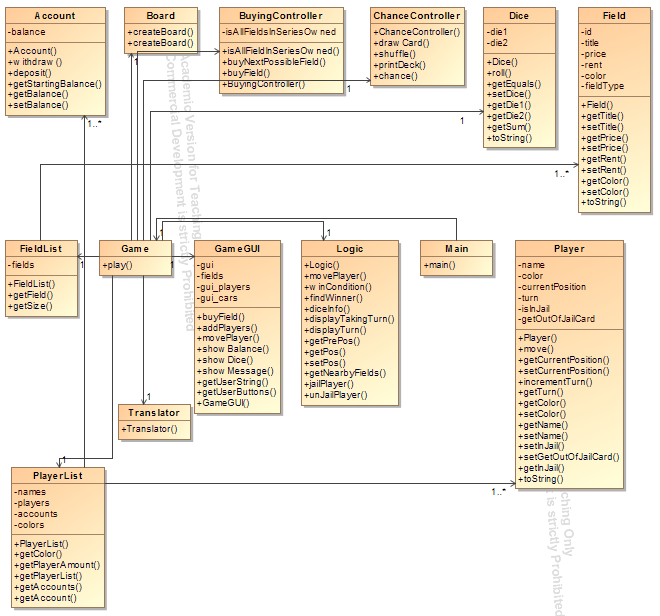
\includegraphics[width=17cm]{sources/6_design/designklassediagram.PNG}
    \caption{Designklassediagram over spil}
    \label{fig:designklassediagram}
\end{figure}

\subsection{Systemsekvensdiagram}




\newpage
\rhead{Implementering}
\section{Implementering} \label{ch7}
Spillet er blevet implementere i Java, der er et objektorienteret programmeringssprog.
Klasserne og metoderne er blevet defineret og implementeret udfra domænemodellen (figur \ref{fig:domænemodel} side \pageref{fig:domænemodel}), designklassediagrammet (figur \ref{fig:designklassediagram} side \pageref{fig:designklassediagram}), og sekvensdiagrammet (figur \ref{fig:Sekvensdiagram} side \pageref{fig:Sekvensdiagram}).

\subsection{BuyingController}
I BuyingController klassen er der et par metoder i spil. Vi har en boolean "isALLFieldsInSeriesOwned". Den tjekker om begge grunde af samme farve er ejet, når spilleren lander på et af de to felter. For at dette kan lade sig gøre, så tjekker den spillerens position (den grund, som spilleren står på) og felterne ved siden af, samt den farve de har. Der efter kigger den på om spilleren ejer begge felter (da det fordobler huslejen for feltet, når en modspiller lander på feltet). Hvis spilleren ikke ejer begge felter (fordi det andet felt er solgt eller ikke ejes endnu), så bliver vores boolean falsk, og resulterer dermed ikke i fordoblet husleje. Dette kan ses på billedet nedenfor:

\begin{figure}[H]
    \centering
    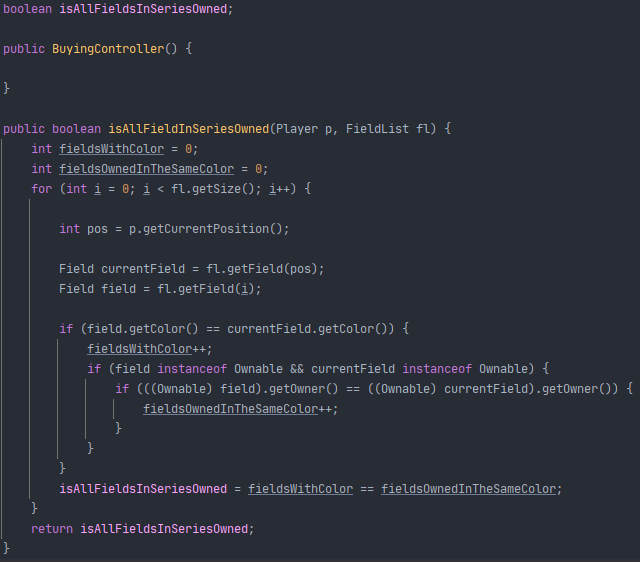
\includegraphics[width=0.7\textwidth]{sources/7_implementering/BuyingController.PNG}
    \caption{Metode der tjekker, om spilleren ejer begge felter af samme farve}
    \label{fig:chance}
\end{figure}

Den næste metode er "buyNextPossibleField". Her tjekker metoden for det næste mulige felt, som ikke er ejet af nogle spillere. Når det felt er fundet, så rykkes spilleren over til det felt, og køber det. Den rykker selvfølgelig spilleren i den rigtige retning rundt på spillepladen. Det er gjort ved en forkommando, som tager udganspunkt i spillerens nuværende position, og derefter tjekker de næste felter, for at se om de kan købes (ownable). Dette kan ses på billedet nedenfor
\begin{figure}[H]
    \centering
    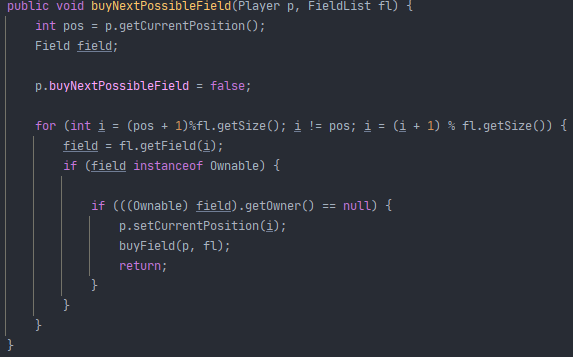
\includegraphics[width=0.7\textwidth]{sources/7_implementering/BuyingControllerMethod2.PNG}
    \caption{Rykker spilleren til det næste mulige felt, og køber der}
    \label{fig:chance}
\end{figure}

Den sidste metode er "buyField". Denne metode gør det muligt for spilleren at købe et ledigt felt. Det gøres ud fra spillerens position, hvor metoden tjekker om det er et felt der kan købes. Hvis feltet kan købes, så går metoden ind i "player" klassen og hæver det beløb, som er tilknyttet feltet. Hvis feltet allerede er solgt til en anden spiller, så tager metoden fat i metoden "isAllFieldInSeriesOwned", for at som om spilleren har været så uheldig, at spilleren skal betale den dobbelte husleje. Hvis der ikke er dobbelt husleje, så betaler spilleren den normale pris til ejeren af feltet. Dette kan ses på billedet nedenfor:
\begin{figure}[H]
    \centering
    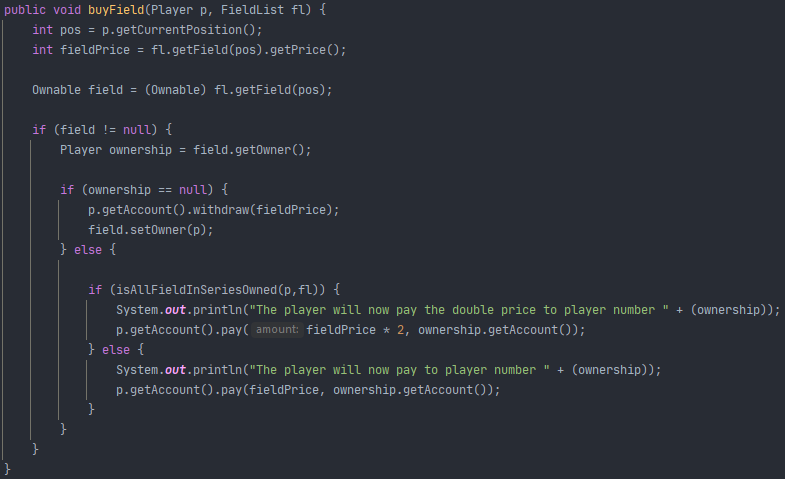
\includegraphics[width=0.7\textwidth]{sources/7_implementering/buyField.PNG}
    \caption{Metode for at sælge felter og tjekke husleje}
    \label{fig:chance}
\end{figure}


\subsection{ChanceController}
\begin{figure}[H]
    \centering
    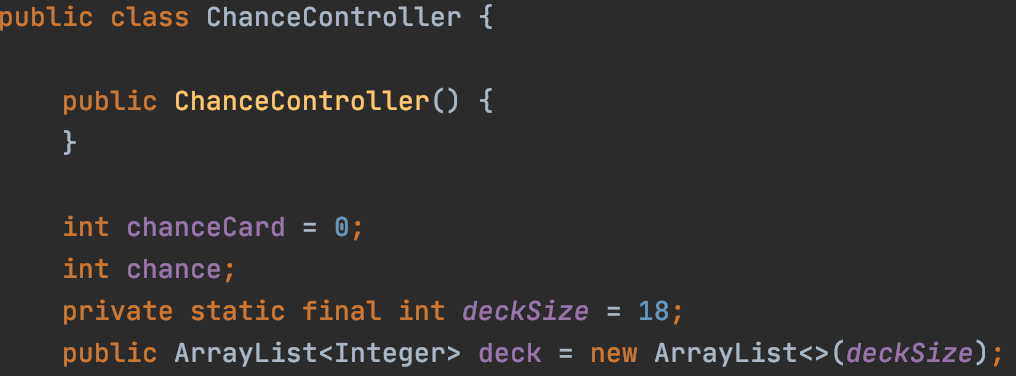
\includegraphics{sources/7_implementering/ControllerClass.png}
    \caption{Vores variable i ChanceController klassen}
    \label{fig:ChanceController}
\end{figure}
I ChanceController klassen har vi to integers, chanceCard og chance. Vores final int deckSize bruger vi til vores chancekort, som vi danner en bunke af ved hjælpe af vores ArrayList.




\begin{figure}[H]
    \centering
    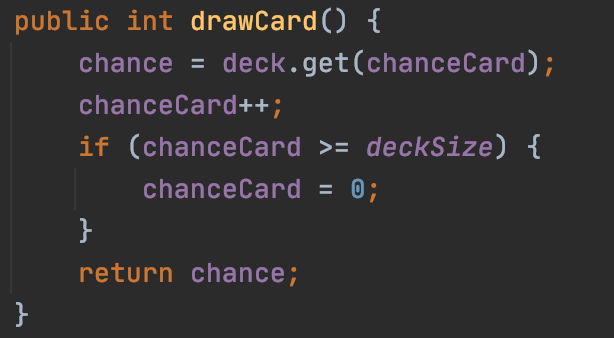
\includegraphics{sources/7_implementering/ControllerDraw.png}
    \caption{Metode til at trække et chancekort}
    \label{fig:draw}
\end{figure}
drawCard metoden bruges til at trække det øverste kort i vores bunke, som vi lavede med ArrayList. Dette fortsætter indtil chance-nummeret bliver lige så højt som vores deckSize, da dette angiver vores kortbunke. Når vi når bunden af bunken, starter den forfra osv.





\begin{figure}[H]
    \centering
    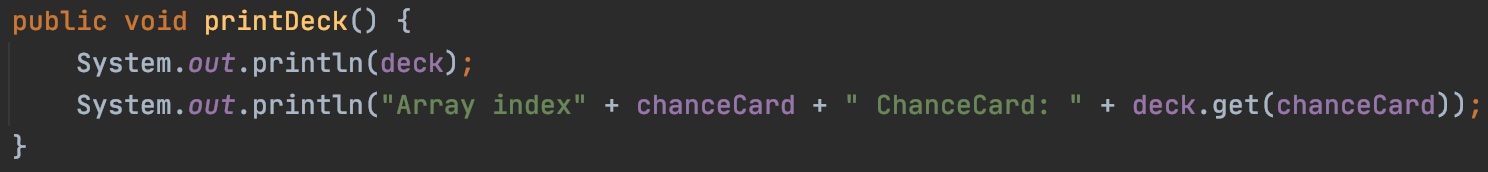
\includegraphics[width=0.7\textwidth]{sources/7_implementering/ControllerprintDeck.png}
    \caption{Metode til at printe dækket og holde styr på bunken}
    \label{fig:print}
\end{figure}
printDeck metoden printer vores dæk i terminalen. Når et nyt chancekort bliver trukket, printer den i terminalen hvilket nummer i arrayet, der blev trukket, og hvilket chancekort (i case rækkefølgen) dette kort er.




\begin{figure}[H]
    \centering
    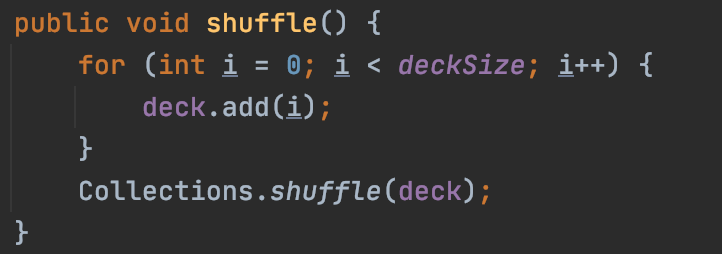
\includegraphics{sources/7_implementering/Controllershuffle.png}
    \caption{Når kortene i bunken skal blandes}
    \label{fig:shuffle}
\end{figure}
Shuffle metoden blander vores chancekort i en tilfældig rækkefølge og danner dermed en bunke.



\begin{figure}[H]
    \centering
    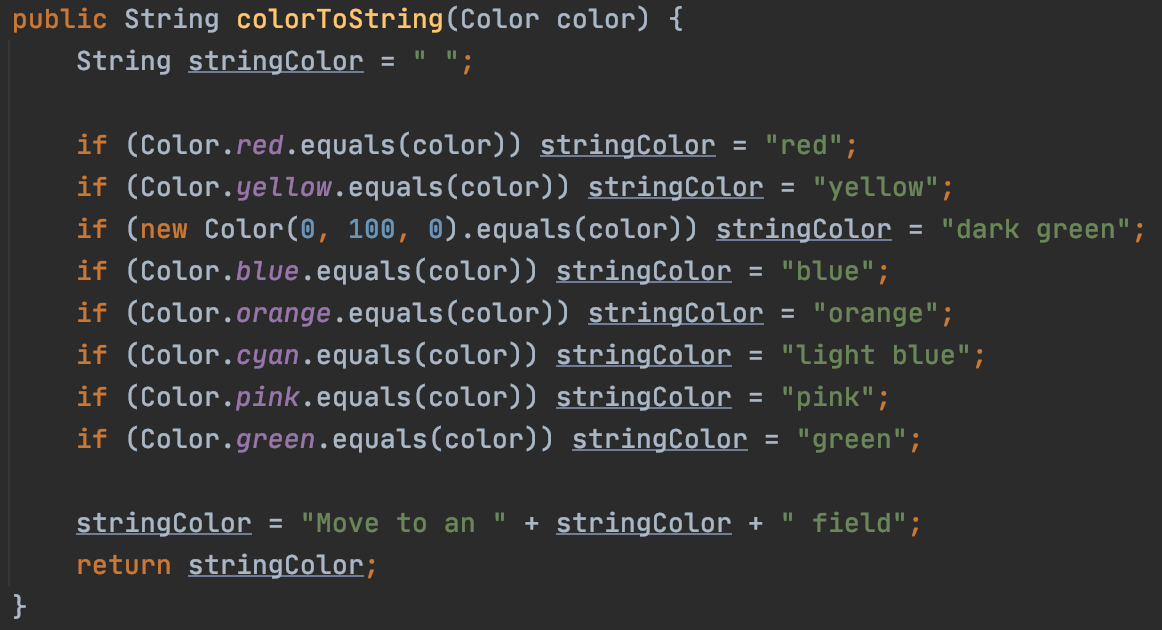
\includegraphics[width=0.7\textwidth]{sources/7_implementering/ControllercolortoString.png}
    \caption{Omdan strings til farve}
    \label{fig:colorString}
\end{figure}
stringColor metoden bruges til at danne strings af alle de farver, som de forskellige felter kan have. Alt efter hvilken farve, man skal lande på, bliver det skrevet på en string.



\begin{figure}[H]
    \centering
    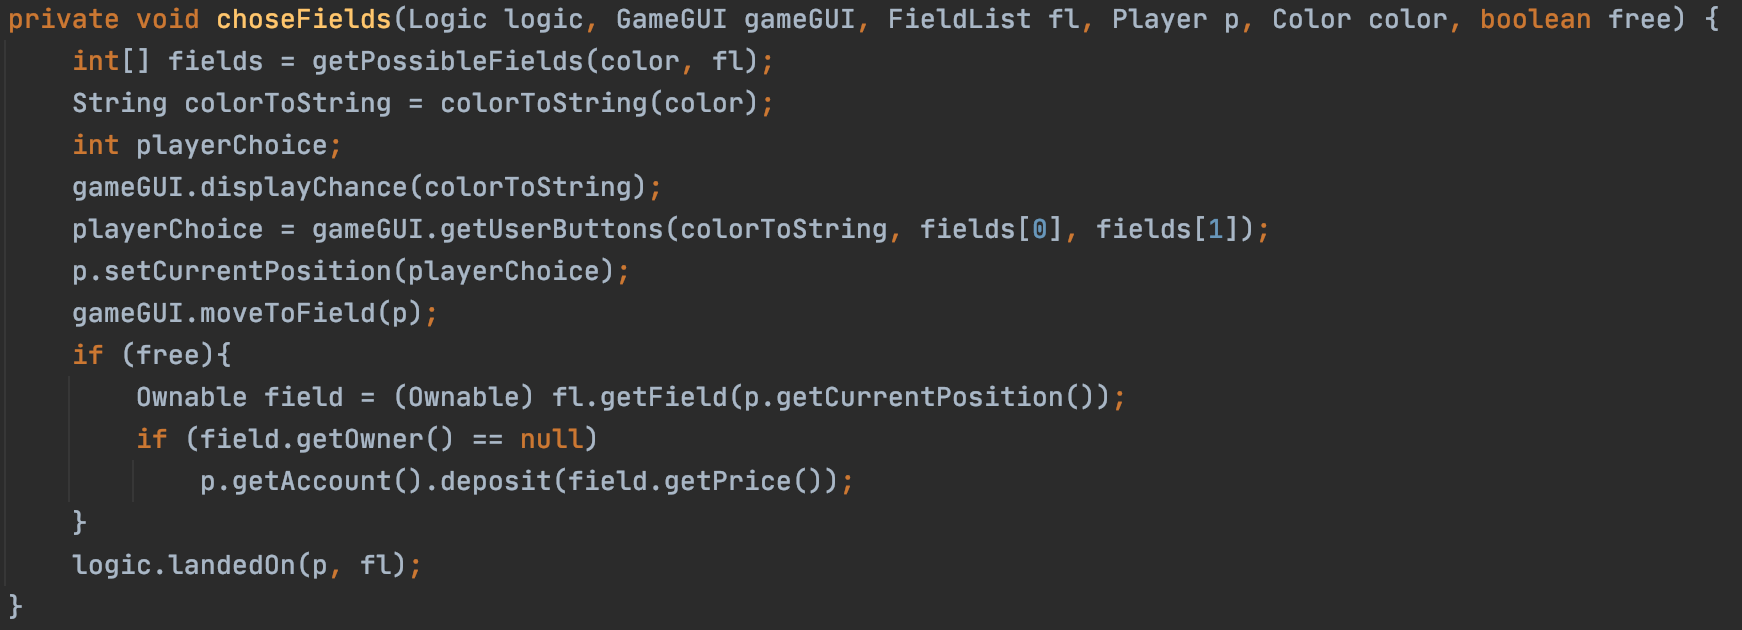
\includegraphics[width=0.7\textwidth]{sources/7_implementering/ControllerchooseFields.png}
    \caption{Vælg et felt af en bestemt farve, man vil rykke til}
    \label{fig:chooseFields}
\end{figure}
chooseFields metoden bruger vi til at vælge et felt, som man vil flytte til. Dette sker i de chance kort, hvor man kan flytte til et felt med en bestemt farve. Metoden holder ligeledes øje med, om feltet er ejet eller frit, da man i så fald skal betale eller købe feltet, man lander på. Metoden sørger også for, at vise dette i GUI’en med displayChance metoden.



\begin{figure}[H]
    \centering
    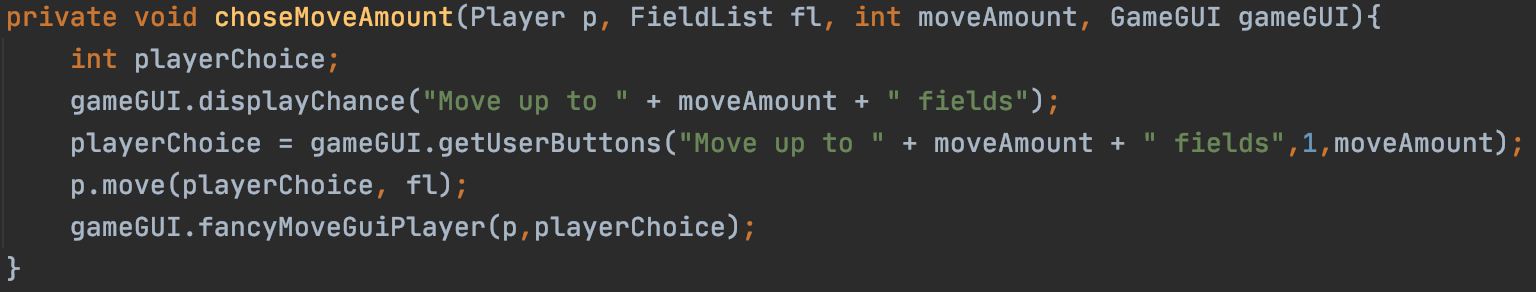
\includegraphics[width=0.7\textwidth]{sources/7_implementering/ControllerMoveAmount.png}
    \caption{Metode til at vælge antal skridt man vil tage}
    \label{fig:MoveAmount}
\end{figure}
chooseMoveAmount metoden bruges til at vælge hvor mange skridt, man vil tage, op til moveAmount. Altså kan spilleren, hvis moveAmount er 10, vælge at rykke ét til 10 felter frem.



\begin{figure}[H]
    \centering
    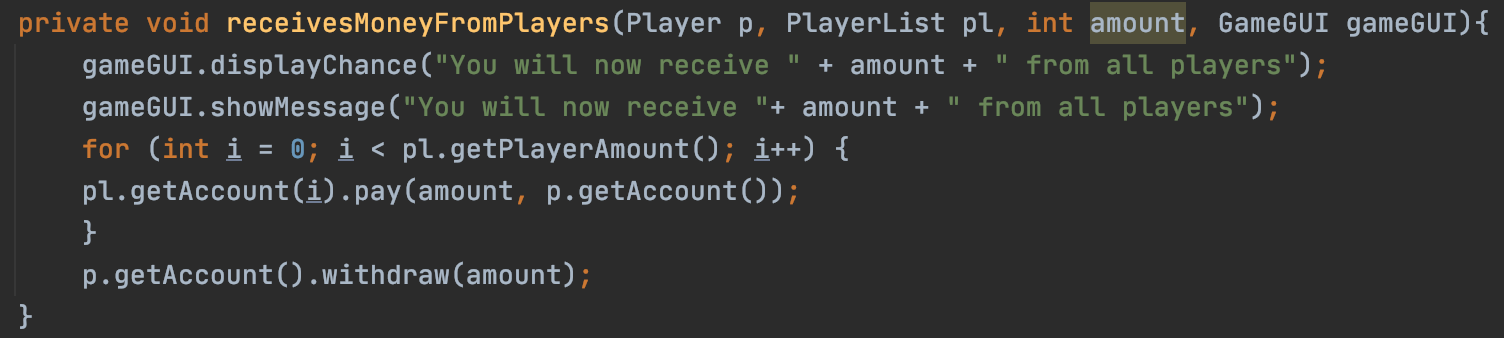
\includegraphics[width=0.7\textwidth]{sources/7_implementering/ControllerRecieveMoney.png}
    \caption{Hvis en spiller skal modtage penge fra andre spilleres konti}
    \label{fig:recieveMoney}
\end{figure}
Denne metode gør, at en spiller modtager penge fra alle andre spillere. Det sker ved, at loopet kører gennem alle spillere, som så får frataget  en bestemt mængde penge, som den éne spiller modtager.



\begin{figure}[H]
    \centering
    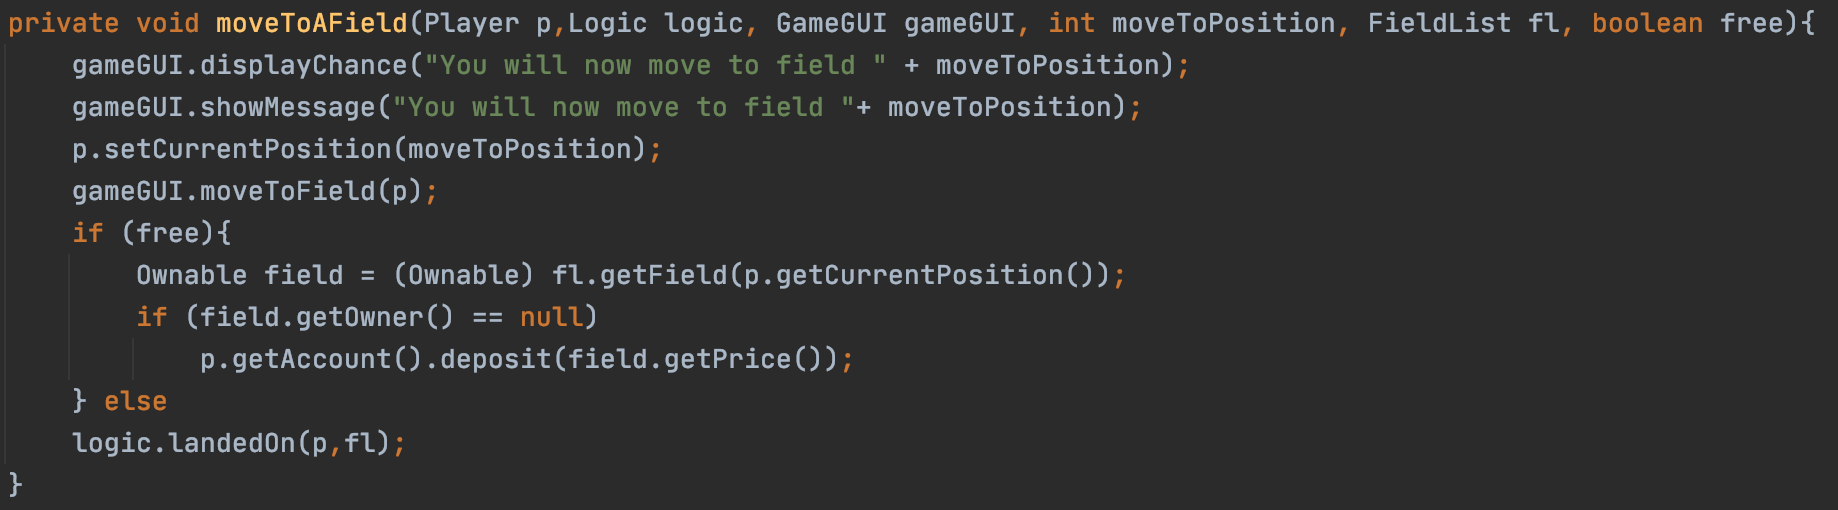
\includegraphics[width=0.7\textwidth]{sources/7_implementering/ControllermoveToField.png}
    \caption{Hvis spilleren skal bevæge sig til et bestemt felt}
    \label{fig:chance}
\end{figure}
I metoden her, bliver spilleren flyttet til et bestemt feltnummer. Når spilleren lander på feltet, tjekker metoden, om feltet kan købes og i så fald, om det er ledigt eller ej.



\begin{figure}[H]
    \centering
    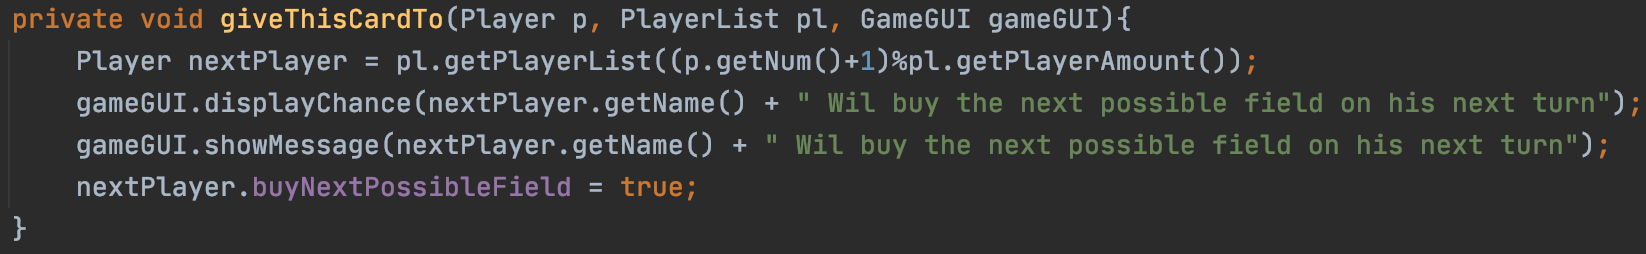
\includegraphics[width=0.7\textwidth]{sources/7_implementering/ControllerGiveCard.png}
    \caption{Metode til at give et kort til en den næste spiller}
    \label{fig:giveCard}
\end{figure}
giveThisCardTo giver et chancekort videre til den spiller, som har næste tur. Denne spiller køber det næste felt, som er ledigt. Dette sker ved buyNextPossibleField metoden.





\begin{figure}[H]
    \centering
    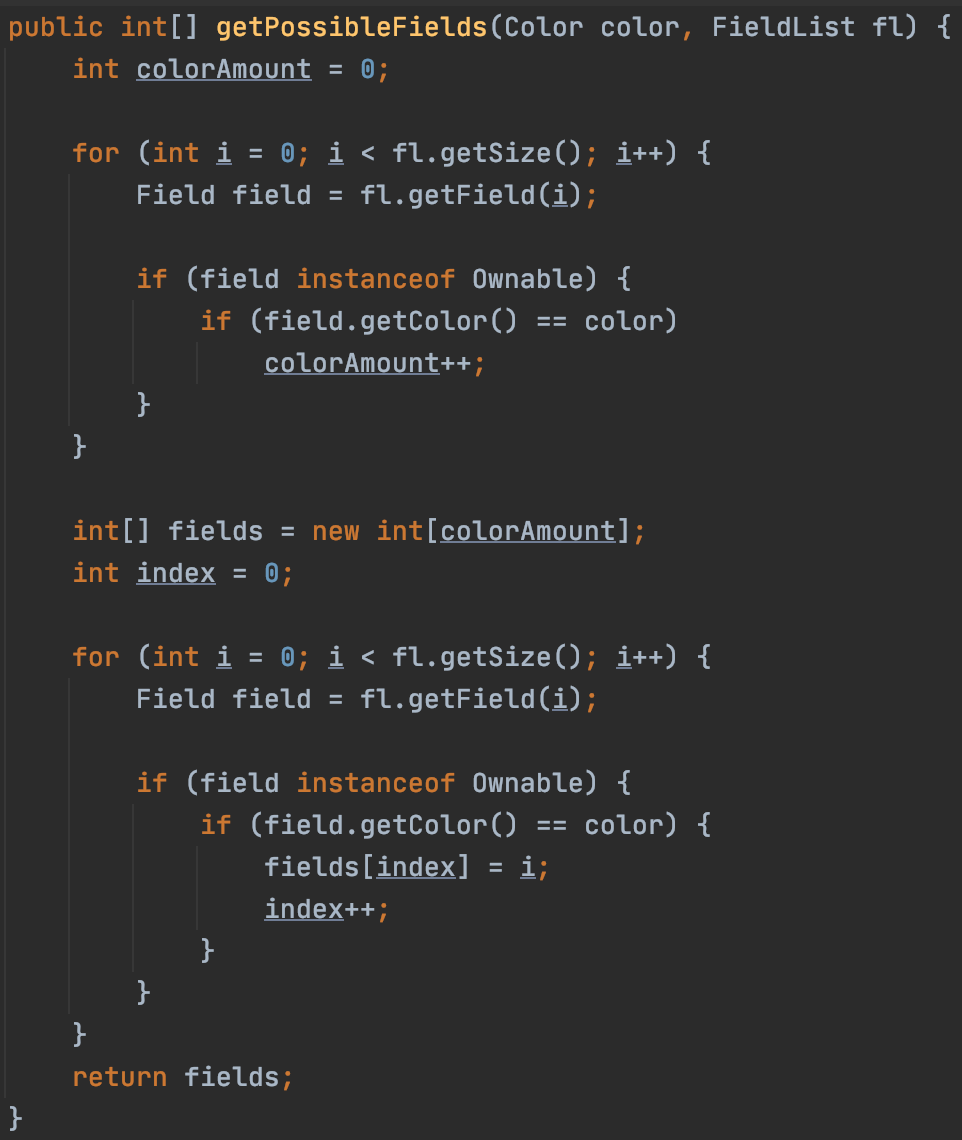
\includegraphics{sources/7_implementering/ControllerGetFields.png}
    \caption{Metode til at se felter af forskellig farve}
    \label{fig:possibleFields}
\end{figure}
Denne metode tjekker hvilke felter, der er af de forskellige farver. Den bruges i chooseFields metoden, når en spiller skal vælge et felt af en speciel farve, som de vil lande på.


\begin{figure}[H]
    \centering
    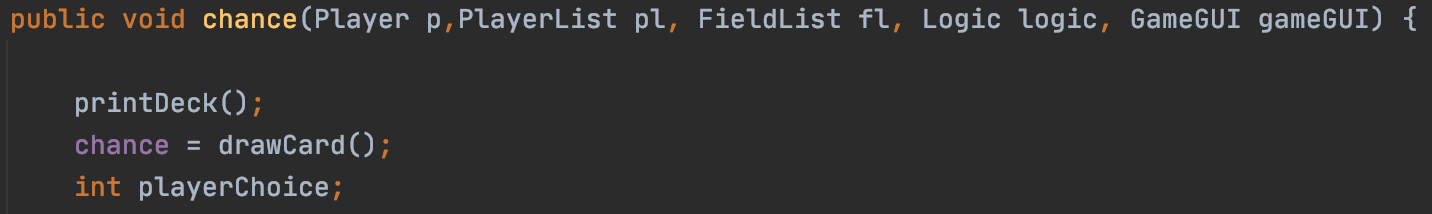
\includegraphics[width=0.7\textwidth]{sources/7_implementering/ControllerChance.png}
    \caption{Metode, som printer dæk og trækker kort når man lander på chancefelt}
    \label{fig:controllerChance}
\end{figure}

chance metoden printer dækket og trækker et kort for en spiller. Denne metode kaldes, når en spiller lander på et chancefelt. 

\begin{figure}[H]
    \centering
    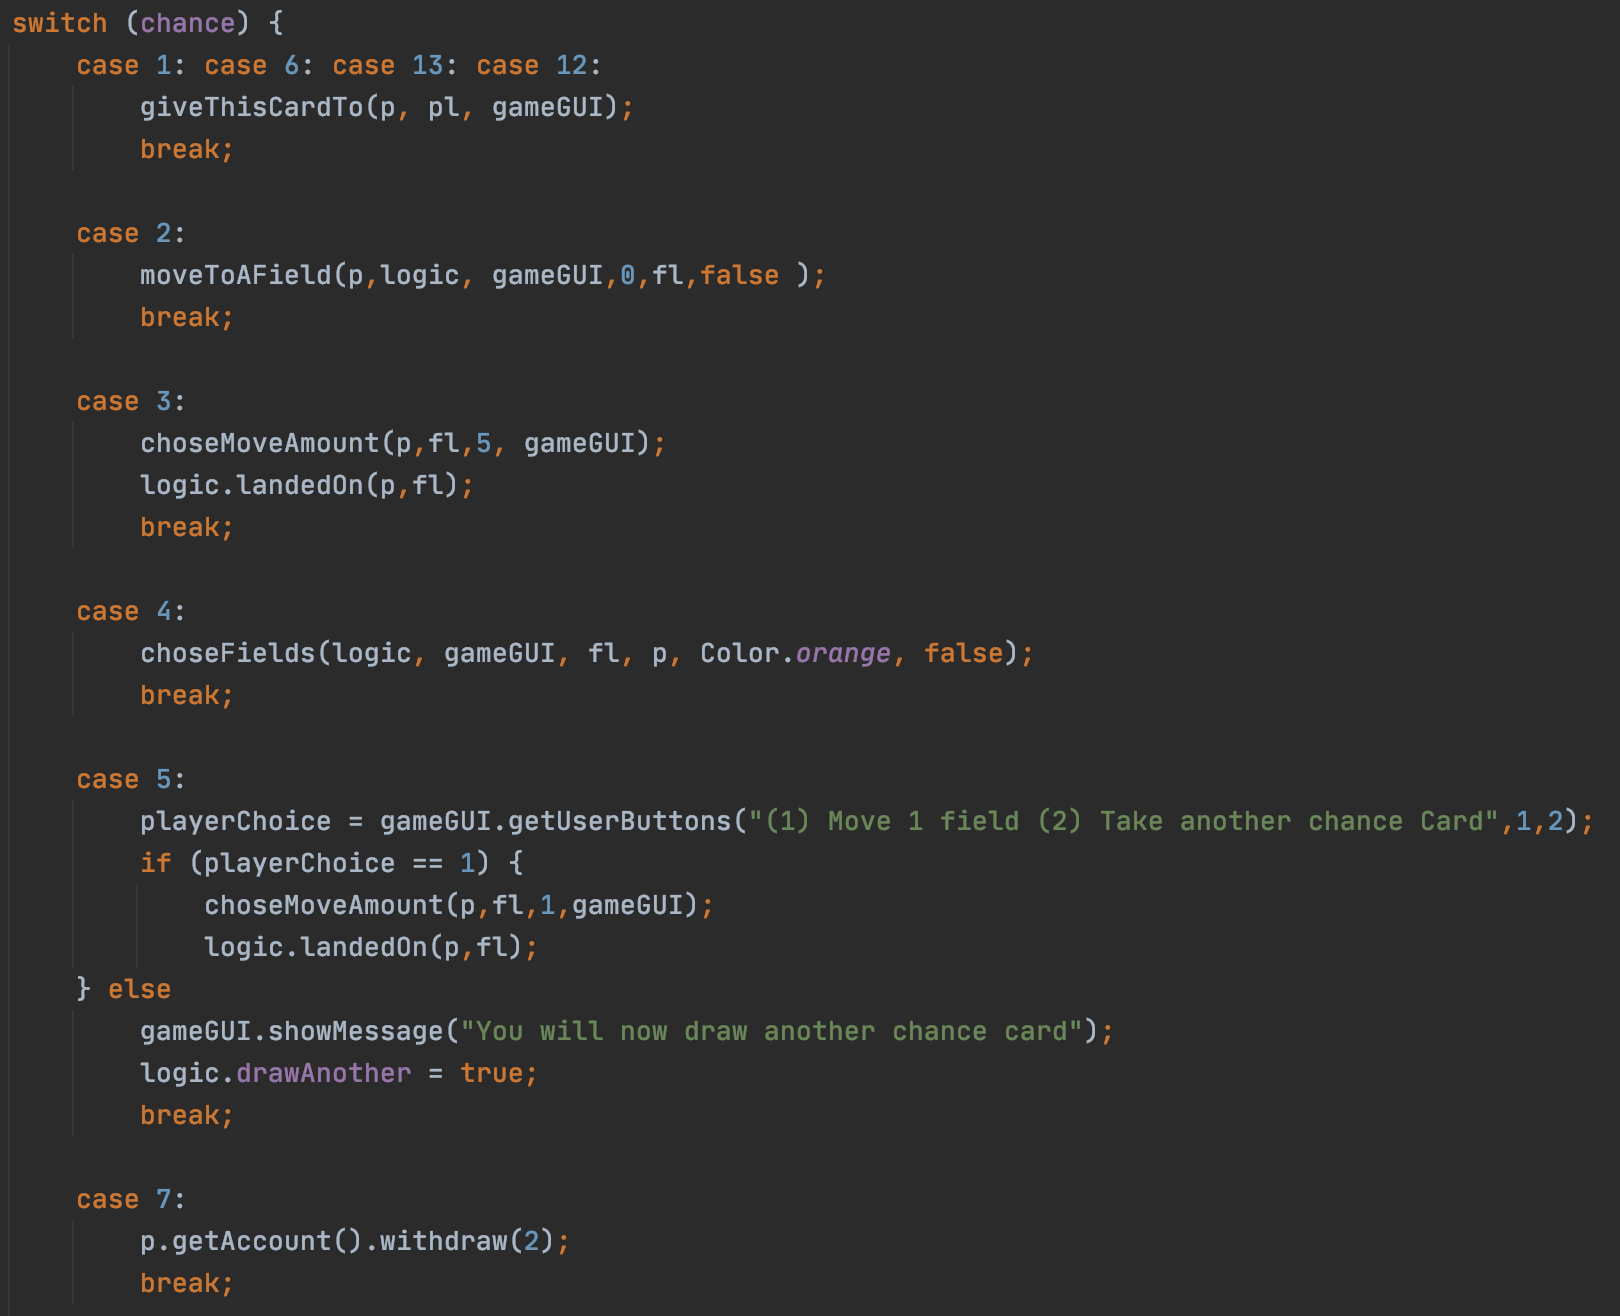
\includegraphics[width=0.7\textwidth]{sources/7_implementering/ControllerChanceSwitch.png}
    \caption{Switch-case til chancekort}
    \label{fig:ControllerChanceSwitch}
\end{figure}
Til slut har vi en længere switch-case, som repræsenterer de forskellige chancekort, som er blevet implementeret. Der er i alt 18 chancekort.














\subsection{Game}
I "Game" klassen er der hvor spillet kører (while loop). Loopet kører indtil der er blevet fundet en vinder udfra "Logic" klassens vinde betingelse. 
\begin{figure}[H]
    \centering
    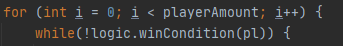
\includegraphics{sources/7_implementering/gameLoop.PNG}
    \caption{"While loop" indtil en vinder er fundet}
    \label{fig:mainLoop}
\end{figure}

Det er også at Chancekort bliver trukket til spillerne fra chancekort dækket(klassen).

\begin{figure}[H]
    \centering
    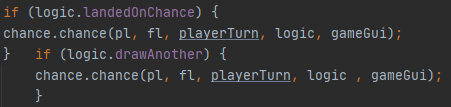
\includegraphics{sources/7_implementering/gameChance.PNG}
    \caption{Hvis spilleren er landet på et chancefelt træk da et chancekort}
    \label{fig:chance}
\end{figure}


\subsection{Logic}
Logic indeholder alt logikken i spillet dvs. de metoder som bliver brugt i "Game" klassen til f.eks. at flytte spillerne, købe felter, eller sætte spilleren i fængsel. Derudover holder klassen også styr på hvad der skal til for at vinde spillet og for at finde vinderen af spillet. Klassen bruges også til at skrive bestemt information ud i konsollen. 


\begin{figure}[H]
    \centering
    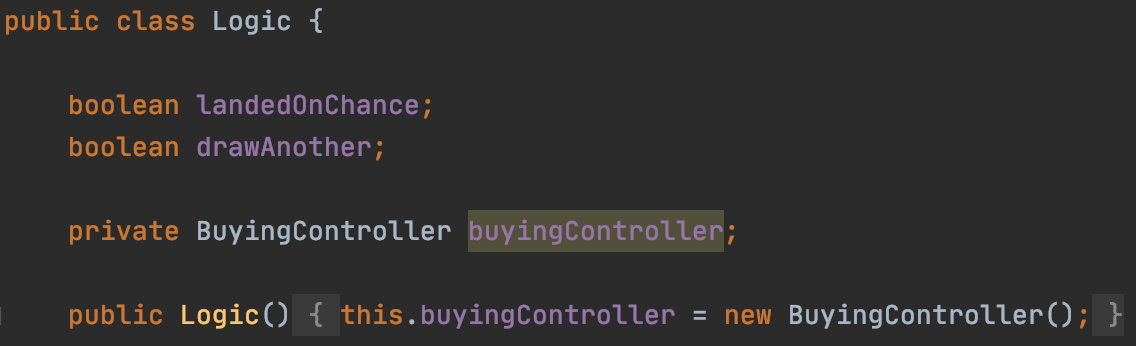
\includegraphics{sources/7_implementering/LogicClass.png}
    \caption{Logic klassen}
    \label{fig:logicClass}
\end{figure}
I klassen har vi defineret to booleans som checker, om man er landet på chance og om man skal trække endnu et kort (drawAnother hører til et bestemt chancekort). Derudover er der en controller til køb og dertil en logic klasse.

\begin{figure}[H]
    \centering
    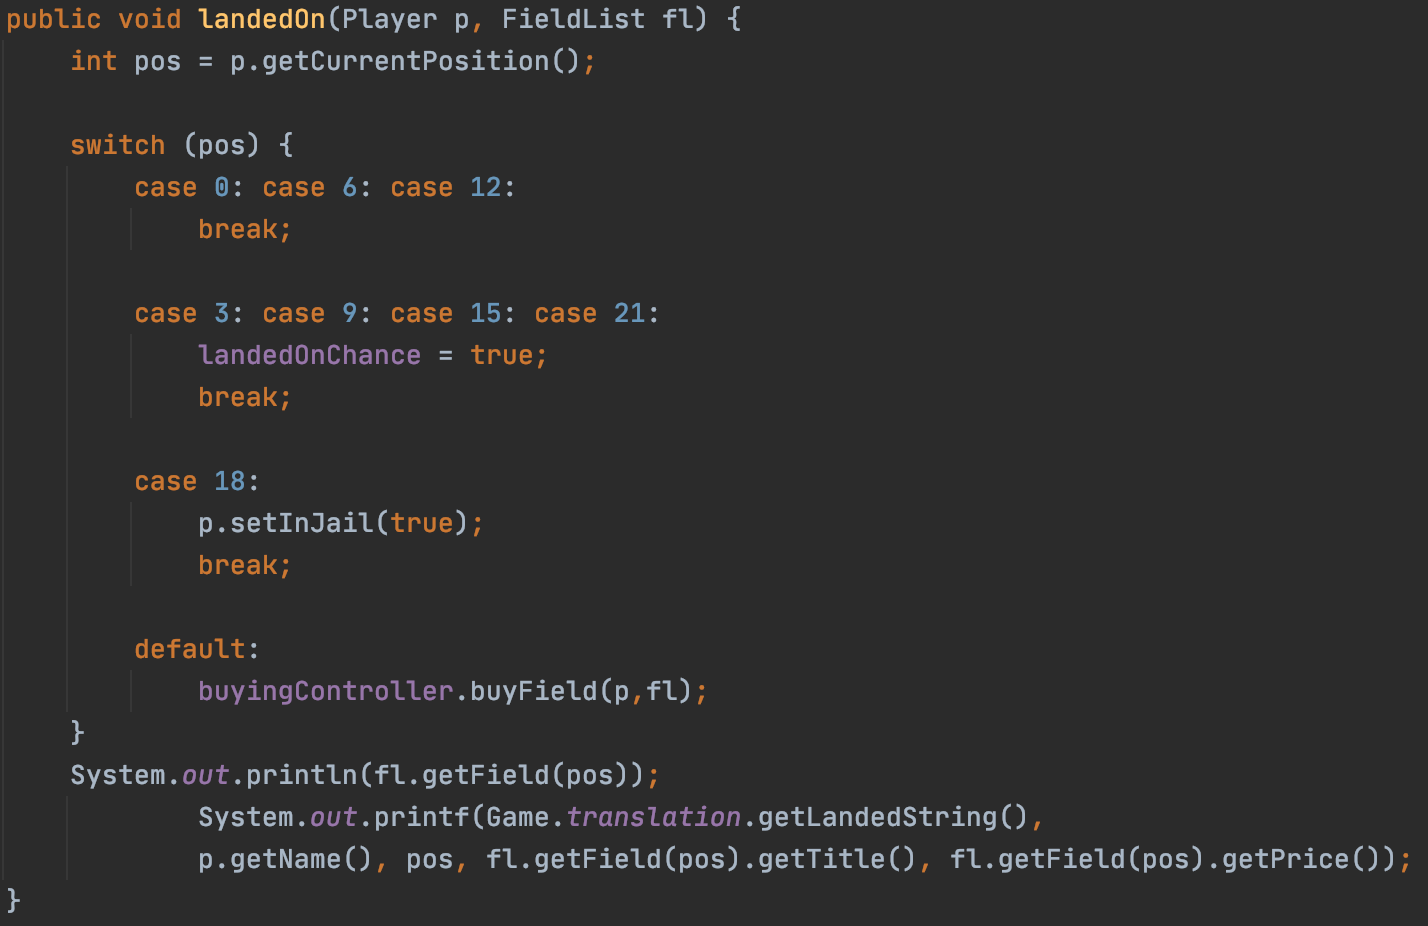
\includegraphics{sources/7_implementering/LogiclandedOn.png}
    \caption{Metoden finder ud af hvilket felt, spilleren lander på}
    \label{fig:logicLandedOn}
\end{figure}
landedOn metoden holder styr på om man er landet på et felt man kan købe, et chancekort eller på fængslet. I så fald vil man blive sat i fængsel, trække et chancekort eller betale for/købe feltet. 



\begin{figure}[H]
    \centering
    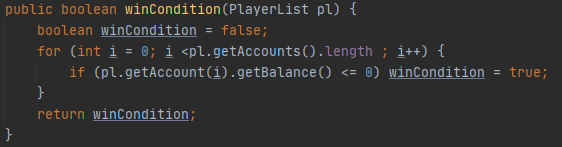
\includegraphics{sources/7_implementering/logic_wincondition.PNG}
    \caption{Når en konto rammer 0}
    \label{fig:logicWinCon}
\end{figure}
winCondition ved, når en spiller har tabt, altså når en konto rammer 0.

\begin{figure}[H]
    \centering
    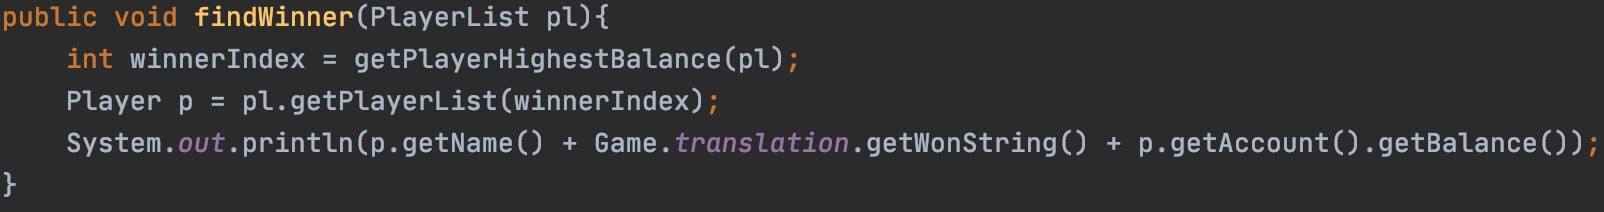
\includegraphics{sources/7_implementering/LogicfindWinner.png}
    \caption{Finder vinderen af spillet}
    \label{fig:logicFindWinner}
\end{figure}
Efter en spiller har tabt, vil metoden her bruge getPlayerHighestBalance metoden og se, hvem der ejer mest. Den vil så erklære vinderen.

\begin{figure}[H]
    \centering
    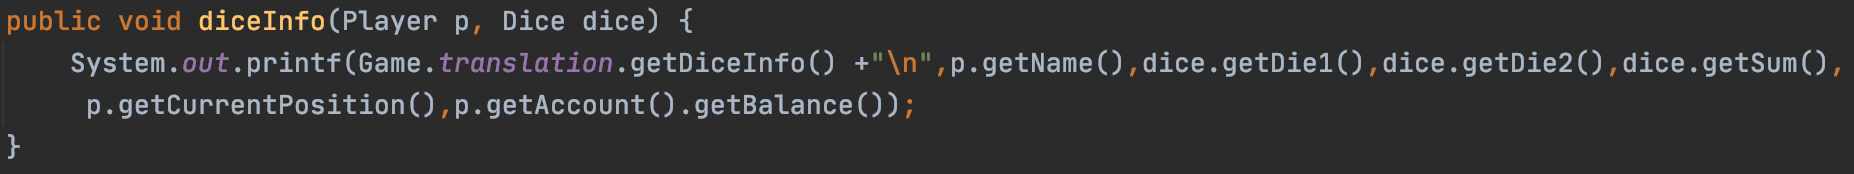
\includegraphics{sources/7_implementering/LogicdiceInfo.png}
    \caption{Metoden viser resultat af terningslag og spillers info efter slag}
    \label{fig:logicDiceInfo}
\end{figure}
diceInfo kalder en række getters . Den får de to terningers øjne og summen af den. Derefter finder den spillerens ny position og kontobeholdning. 

\begin{figure}[H]
    \centering
    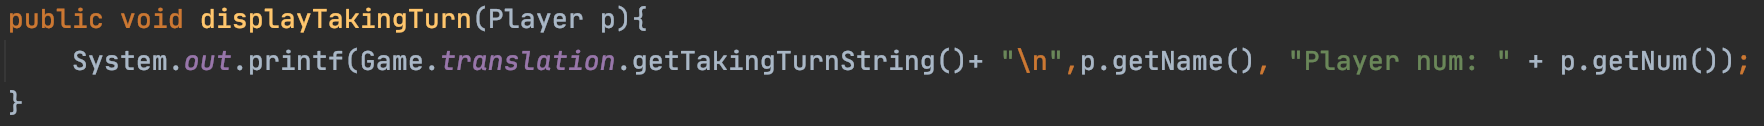
\includegraphics{sources/7_implementering/LogicTakingTurn.png}
    \caption{Kode der beskriver hvordan man vinder}
    \label{fig:logicDisplayTakingTurn}
\end{figure}
displayTakingTurn kender til hvilken spiller, som tager den nuværende tur.

\begin{figure}[H]
    \centering
    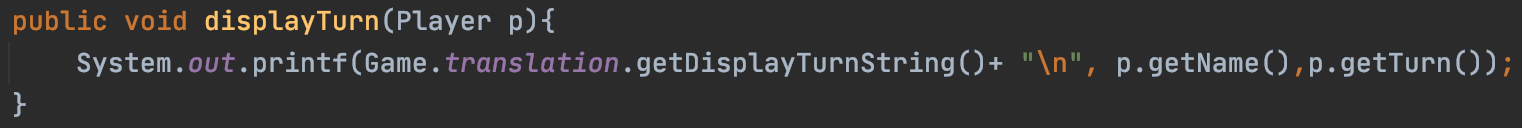
\includegraphics{sources/7_implementering/LogicdisplayTurn.png}
    \caption{Kode der beskriver hvordan man vinder}
    \label{fig:logicDisplayTurn}
\end{figure}
displayTurn fungerer på samme måde og ved hvilken tur, det er.

\begin{figure}[H]
    \centering
    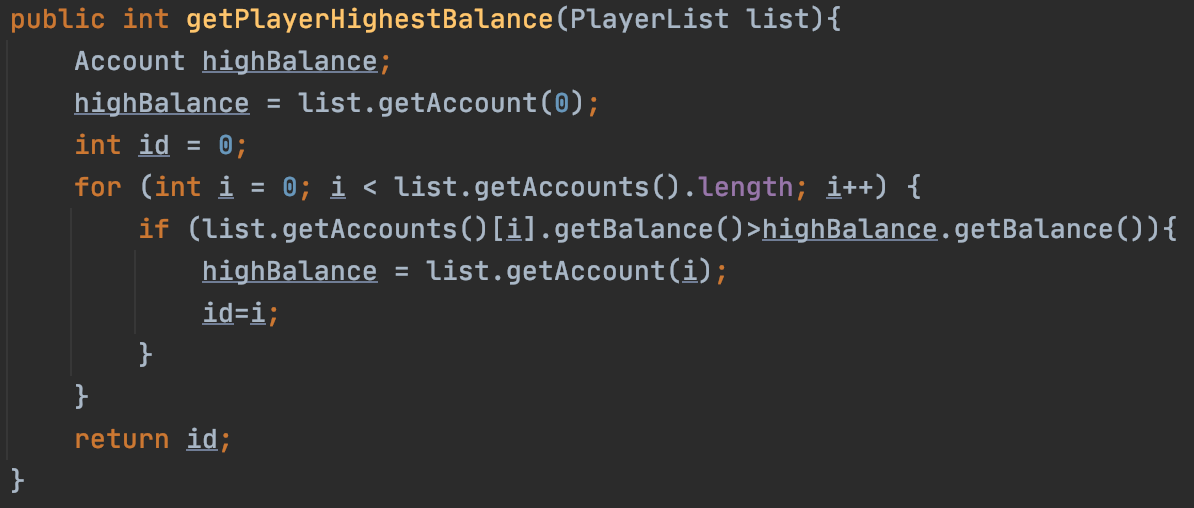
\includegraphics{sources/7_implementering/LogicgetHighestBalance.png}
    \caption{Kode der beskriver hvordan man vinder}
    \label{fig:logicHighestBalance}
\end{figure}
getPlayerHighestBalance bruges til at finde ud af hvilken spiller, der har flest penge på sin konto. Det sker ved et loop, som kigger på alle konti og vælger den med flest penge, som dermed vinder spillet.



\subsection{Main}
I "Main"-klassen starter vi spillet ved at instantiere et objekt af typen game, og bruge metoden play.

\begin{figure}[H]
    \centering
    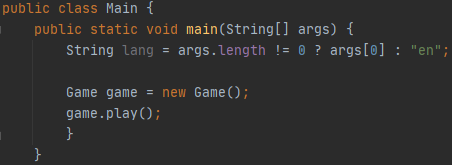
\includegraphics{sources/7_implementering/MainBillede1.png}
    \label{fig:logicWin}
\end{figure}

\subsection{Chance}
Chance-klassen er nedarvet fra "Field" men har derudover også et billede tilknyttet.
\begin{figure}[H]
    \centering
    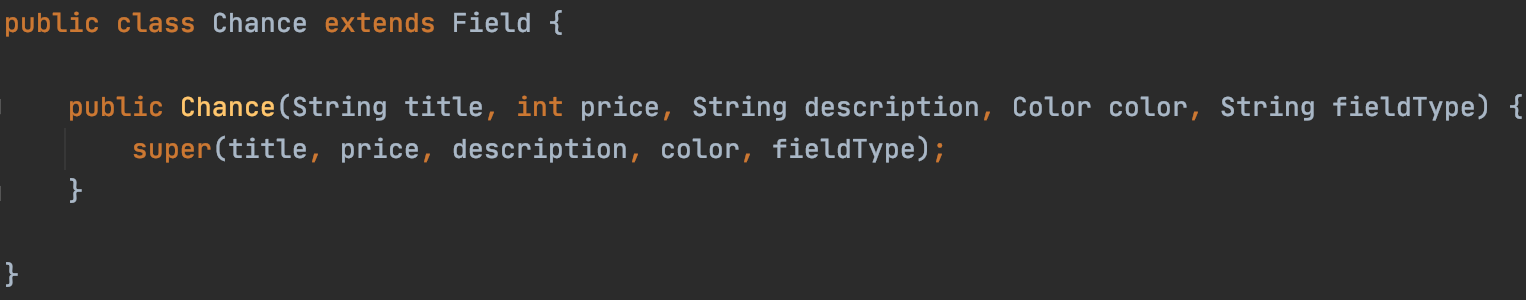
\includegraphics{sources/7_implementering/ChanceField.png}
    \caption{Chance klassen, som er en nedarvet field klasse}
    \label{fig:ChanceField}
\end{figure}

\subsection{Field}
"Field" klassen er en abstrakt klasse, dvs. at den ikke er implementeret. Klassen er abstrakt da der i spillet bliver anvendt mange forskellige slags felter, der mere eller mindre har de samme egenskaber, dog med enkelte variationer. Der er derfor mulighed for at oprette felt klasser der passer speficikt til den type der skal laves. "Field" klassen indeholder en række "standard" metoder som f.eks. en konstruktør (figur \ref{fig:fieldKons}) og en toString() metode (figur \ref{fig:fieldString}).

\begin{figure}[H]
    \centering
    \includegraphics[width=17cm]{sources/7_implementering/fieldkonstruktør.PNG}
    \caption{Field klassens konstruktør}
    \label{fig:fieldKons}
\end{figure}
\begin{figure}[H]
    \centering
    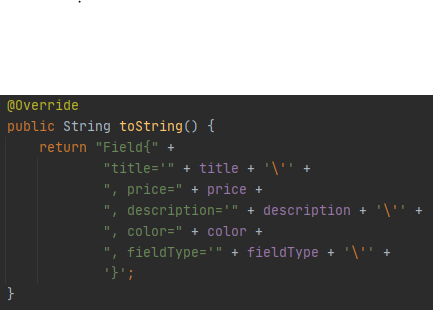
\includegraphics{sources/7_implementering/fieldTostring.PNG}
    \caption{Field klassens toString metode}
    \label{fig:fieldString}
\end{figure}



\subsection{Jail}
"Jail"-klassen er nedarvet fra "Field" men har derudover også et billede tilknyttet.

\begin{figure}[H]
    \centering
    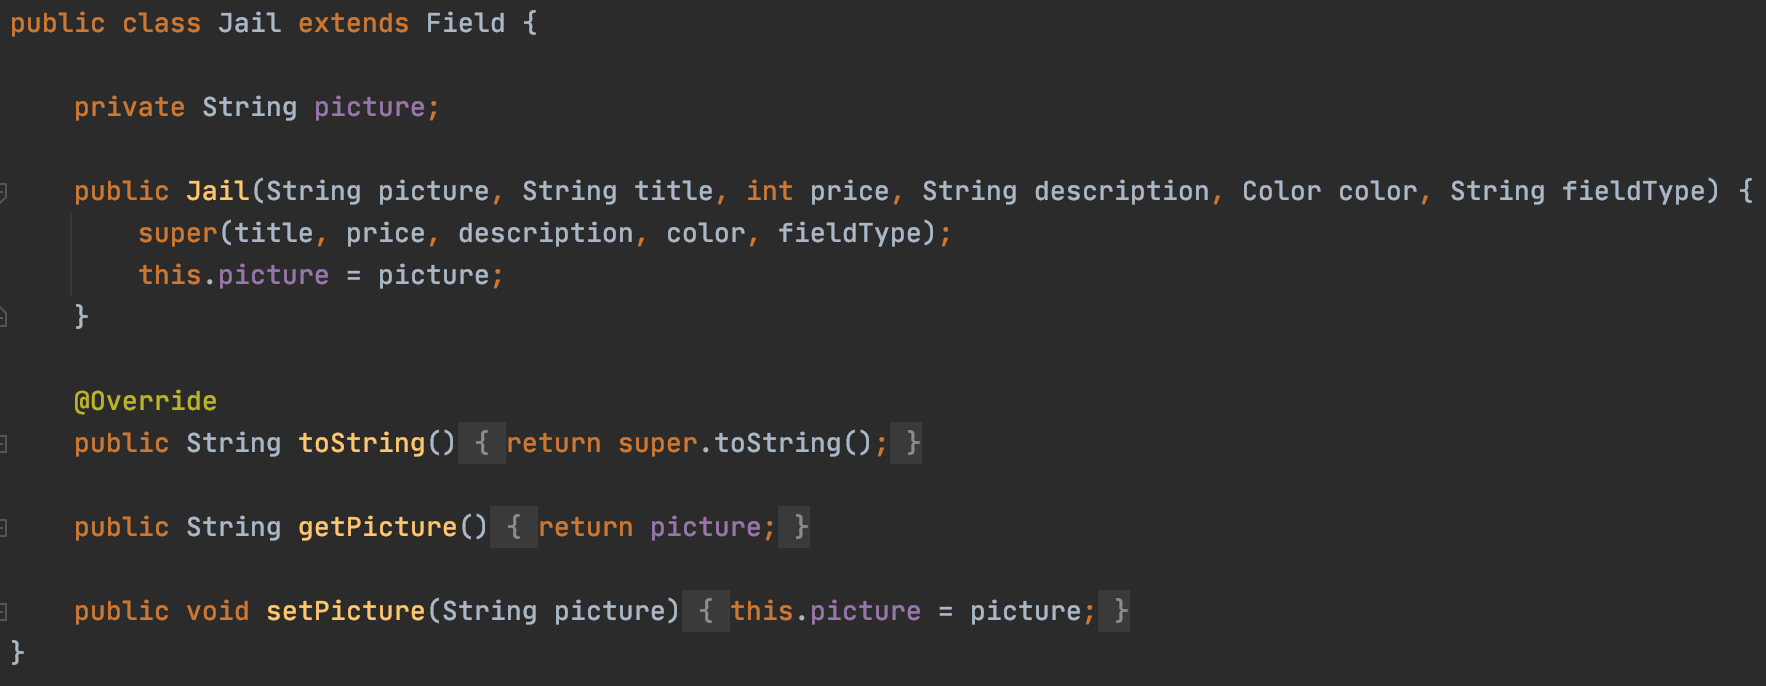
\includegraphics[width=0.7\textwidth]{sources/7_implementering/JailClass.png}
    \caption{Jail klassen}
    \label{fig:Jailklasse}
\end{figure}
Udover de variable, som klassen arver fra field, har den picture, da jail har et specielt billede. Derudover bliver nogle af metoderne overridet, da de stammer fra den abstrakte klasse "Field"

\subsection{Ownable}
"Ownable"-klassen er en abstrakt klasse, der indeholder de atributter, som de felter spillerne kan eje. Klassen er abstrakt, da det ikke skal være muligt at oprette objekter af denne type. Istedet skal de felter der nedarver fra denne klasse oprettes. Klasserne Property, Brewery og Shipping, nedarver alle fra denne klasse. Klassen Ownable indeholder en konstruktør, der tager imod parametrene: title, value, mortgage value og color.
\begin{figure}
    \centering
    \includegraphics{sources/7_implementering/OwnableKonstruktør.PNG}
    \caption{Attributer og konstruktør i Ownable klassen}
    \label{fig:OwnableKons}
\end{figure}
Alle disse paramterer går igen i alle felter der kan ejes. Derudover er atributten Owner af typen "Player" blevet implementeret med en Getter og Setter metode.

\subsection{Parking}
"Parking"-klassen er ligesom "Jail"-klassen nedarvet fra "Field" men har derudover også et billede tilknyttet.

\begin{figure}[H]
    \centering
    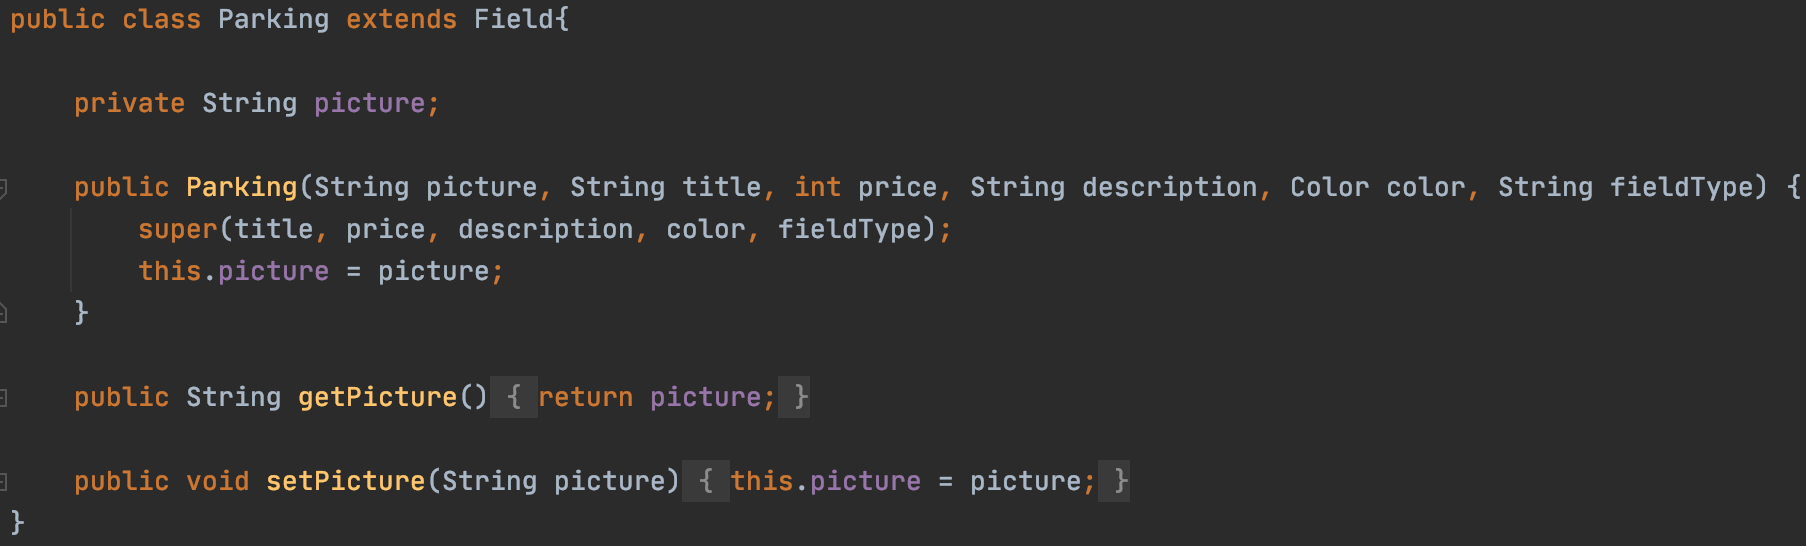
\includegraphics[width=0.7\textwidth]{sources/7_implementering/Parking.png}
    \caption{Parking klasse}
    \label{fig:Parking}
\end{figure}
Parking er en lille udvidelse af fields. Der er ingen konsekvens eller gevinst af at lande på parking, så der bliver blot tilføjet et billede til brug på spilbrættet.

\subsection{Start}
"Start"-klassen er nedarvet fra "Field" men har derudover også et billede tilknyttet.

\begin{figure}[H]
    \centering
    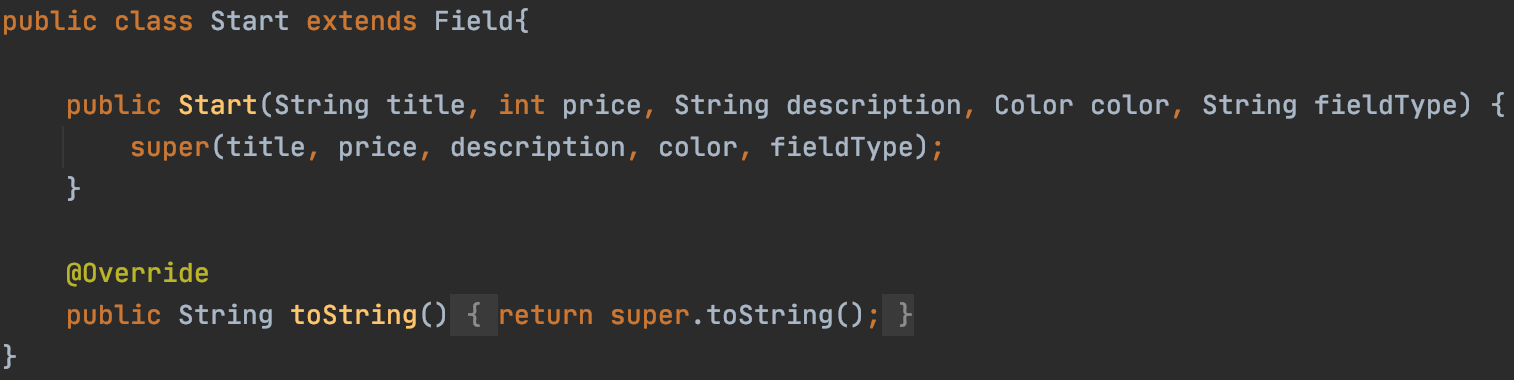
\includegraphics[width=0.7\textwidth]{sources/7_implementering/StartKlasse.png}
    \caption{Start klassen}
    \label{fig:Startklasse}
\end{figure}
Start ejer som de andre felttyper sine variable fra Field, og der defineres ikke nye variable heri.

\subsection{Account}
I "Account" klassen holdes der styr på spillerens mængde af penge. Der kan både hæves og indsættes penge på spillerne konti. Først oprettes spillerens konto. Den mængde penge spilleren bliver tildelt ved starten af spillet, er afhængigt af antallet af spillere, når spillet startes. Det vil vi kommen nærmere ind på senere i denne klasse. Nedenfor kan metoden ses:
\begin{figure}[H]
    \centering
    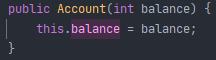
\includegraphics[width=0.7\textwidth]{sources/7_implementering/Account.PNG}
    \caption{Start Beløb}
    \label{fig:chance}
\end{figure}

Derefter kommer metoden "withddraw", som gør det muligt at hæve penge fra spillernes konti. Her er det dog ikke muligt at gå i minus, så ved dette tilfælde sættes spillerens konto til 0:
\begin{figure}[H]
    \centering
    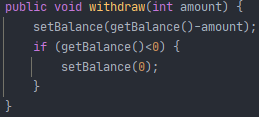
\includegraphics[width=0.7\textwidth]{sources/7_implementering/withdraw.PNG}
    \caption{Metode til at hæve penge}
    \label{fig:chance}
\end{figure}
I denne metode "deposit", kan spillerne moddtage penge. I tilfældet at spilleren konto er i minus, så sættes den til 0 inden beløbet indsættes på kontoen:
\begin{figure}[H]
    \centering
    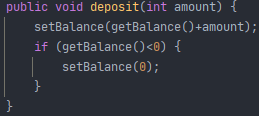
\includegraphics[width=0.7\textwidth]{sources/7_implementering/deposit.PNG}
    \caption{Metode til at indsætte penge}
    \label{fig:chance}
\end{figure}
I metoden "pay", kan spilleren betale husleje til spilleren, som ejer det felt der landes på:
\begin{figure}[H]
    \centering
    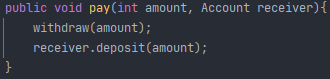
\includegraphics[width=0.7\textwidth]{sources/7_implementering/pay.PNG}
    \caption{Metode til at betale en spiller}
    \label{fig:chance}
\end{figure}
Når et nytspil startes, så tages metoden "getStartingBalance" i brug. Alt afhængigt af antallet af spillere modtager hver spiller et bestemt beløb. Det betyder, at ved 2 spillere, så mådtager hver spiller 20 millioner, ved 3 spiller modtager de hver 13 millioner og ved 4 spillere, modtager de hver 16 millioner. Det beløb den individuelle spiller har kan også kaldes på ved metoden "getBalance":
\begin{figure}[H]
    \centering
    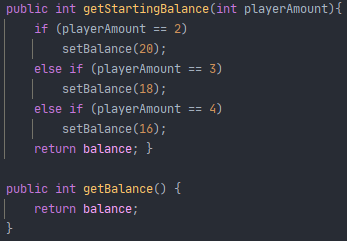
\includegraphics[width=0.7\textwidth]{sources/7_implementering/startBal.PNG}
    \caption{Metode for bestemme startbeløb for spillerne}
    \label{fig:chance}
\end{figure}
Inden spillerne har modtaget et start beløb, så er vi nødt til at definere et beløb til dem. Derfor har de bare 0 millioner, men det har ikke rigtig nongen betydning.
\begin{figure}[H]
    \centering
    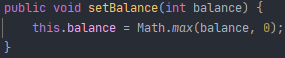
\includegraphics[width=0.7\textwidth]{sources/7_implementering/getBal.png}
    \caption{Midlertidigt startbeløb}
    \label{fig:chance}
\end{figure}


\subsection{Player}
Klassen "Player" holder styr på spillernes tildelte farve, deres navn, nuværende position, deres forige position, om de er i fængsel og har de et chancekort, som kan få dem ud af fængslet. Dette er klaret på en række af metoder.

Vi har en metode "Player", som gør det muligt for spilleren at skrive et navn, få en farve, få tildelt en "account" og hvilken tur spilleren er på. Dette kan ses på følgende billede:
\begin{figure}[H]
    \centering
    \includegraphics[width=0.7\textwidth]{sources/7_implementering/Player.PNG}
    \caption{Player konstruktør}
    \label{fig:PlayerKonstruktør}
\end{figure}
For at spilleren kan rykke rundt på spillepladen, så har vi lavet matoden "move". Inden spilleren rykker til den nye position, så bliver den tidligere position sat til den nuværende. Derefter lægges spillerens nuværende position sammen med det antal øjne der er slået med terningerne. Hvis man slår nok til, at passere startfeltet, så har vi anvendt modulus, så man kan rykke hele vejen rundt:
\begin{figure}[H]
    \centering
    \includegraphics[width=0.7\textwidth]{sources/7_implementering/Move.PNG}
    \caption{Metoder der flytter spilleren}
    \label{fig:PlayerMove}
\end{figure}
Når spillerens tur er overstået, så stiger spillerens "runde-tal" med 1:
\begin{figure}[H]
    \centering
    \includegraphics[width=0.7\textwidth]{sources/7_implementering/Turn.PNG}
    \caption{Metode der holder styr på turen}
    \label{fig:TurnKeeper}
\end{figure}
Derefter har vi en række getters \& setters, som holder styr på farve, navn, konto, om spilleren er i fængsel og kan spilleren komme ud af fængsel:
\begin{figure}[H]
    \centering
    \includegraphics[width=0.7\textwidth]{sources/7_implementering/getSet.PNG}
    \caption{Getters og setters i player klassen}
    \label{fig:GetterSetter}
\end{figure}


\subsection{Dice }
I denne klasse bliver der slået med terningerne.
\begin{figure}[H]
    \centering
    \includegraphics[width=0.7\textwidth]{sources/7_implementering/Dice.PNG}
    \caption{Dice konstruktør}
    \label{fig:DiceKons}
\end{figure}
Dice klassen begyndder med, at vi opretter to die og kalder en roll metode på dem.
\begin{figure}[H]
    \centering
    \includegraphics[width=0.7\textwidth]{sources/7_implementering/Roll.PNG}
    \caption{Roll metoden i Dice}
    \label{fig:diceRoll}
\end{figure}
Roll metoden bruger Random metoden, så når terningerne ‘kastes’ vil de hver have en værdi mellem 1 og 6. Der vil ligeledes blive returneret en sum af de to terningers værdier.
\begin{figure}[H]
    \centering
    \includegraphics[width=0.7\textwidth]{sources/7_implementering/equal.PNG}
    \caption{Getter og setters, samt toString metode}
    \label{fig:Dicemisc}
\end{figure}
Boolean'en getEquals metoden, viser, når vores terninger har samme værdi, da det resulterer i et ekstra kast.
Herefter har vi først en setDice metode, som bruges til at tilvige terningerne en bestemt værdi, og efterfølgende en getDice metode, som kan returnere udfaldet af de to terninger hver især eller deres sum.


\subsection{FieldList}
"fieldList"-klassen indeholder et array med vores 24 spilfelter. Arrayet indeholder felter defineret af vores tidligere nævnte klasser: Ownable, Jail, Parking, Start, Chance. Disse klasser er nedarvet fra "Field"-klasen hvorfra det er bestemt at alle felter har en titel, pris, beskrivelse, farve og type som specificeres i dette array.


\subsection{PlayerList}

vores PlayerList klassse indeholder et array af spillere og deres accounts hver især. Derudover kender den til hvilken spiller, der har turen med currentPlayer og har et ID til hver spiller, f.eks. 1,2,3 for tre spillere.
\begin{figure}[H]
    \centering
    \includegraphics[width=0.7\textwidth]{sources/7_implementering/PlayerListClass.png}
    \caption{De definerede variable i PlayerList klassen}
    \label{fig:playerListklasse}
\end{figure}



\begin{figure}[H]
    \centering
    \includegraphics[width=0.7\textwidth]{sources/7_implementering/PlayerListList.png}
    \caption{PlayerList metode til spilleroprettelse}
    \label{fig:playerListmetode}
\end{figure}
PlayerList klassen laver en liste med alle spillere i spillet.  Den opretter de forskellige spillere, deres accounts og giver dem et nummer hver.


\begin{figure}[H]
    \centering
    \includegraphics[width=0.7\textwidth]{sources/7_implementering/PlayerListGetSet.png}
    \caption{PlayerList Get/Set}
    \label{fig:plistGetSet}
\end{figure}
Til slut er der en række getters og setters for PlayerAmount, Accounts, CuttentPlayer og Next player. Disse holder øje med hvilken spiller. der har turen og man kan dermed få fat på hvilken spiller, der har turen og hvordan deres konto ser ud.


\subsection{GameGUI}
GUI klassen er det grafiske. Her kan vi vise en bil i en bestemt farve som spilleren er blvet tildelt. Der oprettes altså spillere. Dette ses på følgende billede:

\begin{figure}[H]
    \centering
    \includegraphics[width=0.7\textwidth]{sources/7_implementering/GameGUIaddPlayers.png}
    \caption{Bil \& farve tildeles spillerne}
    \label{fig:playerListklasse}
\end{figure}

GameGUI klassen skal bruge en konstuktør. Derfor oprettes følgende konstuktør for vores GUI:
\begin{figure}[H]
    \centering
    \includegraphics{sources/7_implementering/GameGUIclass.png}
    \caption{Konstruktør}
    \label{fig:playerListklasse}
\end{figure}

Når en spiller lander på et chance-kort, så skal kortet med teksten vises til spillerne. Det er gjort ved at kalde på den beske, som er tilknyttet chancekortet, så teksten kan sættes på et "fysisk" chance-kort:
\begin{figure}[H]
    \centering
    \includegraphics{sources/7_implementering/GameGUIdisplayChance.png}
    \caption{Chance-kort besked}
    \label{fig:playerListklasse}
\end{figure}

Metoden "fancyMoveGuiPlayer" og "moveToField" Rykker spillernes brikker med rundt på spillepladen. Dette kan ses på de følgende to billeder: 
\begin{figure}[H]
    \centering
    \includegraphics{sources/7_implementering/GameGUIfancyMove.png}
    \caption{fancyMoveGuiPlayer-klassen}
    \label{fig:GUIklasse}
\end{figure}
moveToField sørger for, at brikken rykker sig til en ny position på spilbrættet.
\begin{figure}[H]
    \centering
    \includegraphics[width=0.7\textwidth]{sources/7_implementering/GameGUImoveToField.png}
    \caption{moveToField-klassen}
    \label{fig:GUImoveToField}
\end{figure}
"showBalance" viser spillerne hvor mange penge de har:
\begin{figure}[H]
    \centering
    \includegraphics{sources/7_implementering/GameGUIshowBalance.png}
    \caption{Balance}
    \label{fig:GUIbalance}
\end{figure}
Når spilleren slår med terningen, så viser denne metode de visuelle kast/resultat:
\begin{figure}[H]
    \centering
    \includegraphics[width=0.7\textwidth]{sources/7_implementering/GameGUIshowDice.png}
    \caption{Terning}
    \label{fig:GUIterning}
\end{figure}
Metoden "showMessage" viser beskederne, som f.eks. spørger spilleren om man vil slå med terningen, købe grunden eller andre lignende beskeder:
\begin{figure}[H]
    \centering
    \includegraphics{sources/7_implementering/GameGUIshowMessage.png}
    \caption{Beskeder}
    \label{fig:GUIbeskeder}
\end{figure}
Når et felt bliver købt, så bliver feltet markeret med ejerens farve i kanten rundt. Det er gjort ved metoden "updateFieldBuy":
\begin{figure}[H]
    \centering
    \includegraphics{sources/7_implementering/GameGUIupdateFieldBuy.png}
    \caption{Ejer af felter}
    \label{fig:GUIfeltEjer}
\end{figure}




\newpage
\rhead{Konfiguration}
\section{Konfiguration} \label{ch9}
\subsection{Versionsstyring}
.

\subsection{Hent og byg spillet}



\newpage
\rhead{Test}
\section{Test} \label{ch10}





\newpage
\rhead{Projektplanlægning}
\section{Projektplanlægning} \label{ch11}
\input{sources/10_projektplanlægning}

\newpage
\rhead{Konklusion}
\section{Konklusion} \label{ch12}
Udfra kundens vision er der blevet opsillet en række krav og use cases, som kunden ville have udført af spillet. Der er udfra kravene og use cases blevet udarbejdet et design over spillet, med tilhørende domænemodel og systemsekvensdiagram. Udfra designet er spillet blevet implementeret i Java. Efterfølgende er der blevet udarbejdet en række test, der har til formål at teste om spillet lever op til kravene. Da der er blevet udarbejdet relativ få test, er det svært at sige om spillet lever op til alle kravene. Udfra fra en vurdering, opfylder Matador spillet  i høj grad kundens vision, om et grundlæggende Matador spil, som har de basale funktioner og virker.




\newpage
\rhead{Figurer}
\addcontentsline{toc}{section}{List of Figures}
\listoffigures
\thispagestyle{fancy}

\newpage
\rhead{Tabeller}
\addcontentsline{toc}{section}{Tabeller}
\listoftables
\thispagestyle{fancy}


\newpage
\rhead{Litteratur}
\addcontentsline{toc}{section}{Litteratur}
\printbibliography

\newpage
\section{Bilag} \label{ch13}
\addcontentsline{toc}{section}{Bilag}
\appendix




\label{endOfDoc}
\end{document}
